\documentclass[tikz,border=6pt]{standalone}
% Shared figure style for the Space Data Network whitepapers.
\usepackage{lmodern}
\usepackage[T1]{fontenc}
\usepackage{xcolor}
\usetikzlibrary{arrows.meta,positioning,calc,fit,backgrounds,matrix}
\hyphenpenalty=10000\exhyphenpenalty=10000
\definecolor{ink}{HTML}{1F2328}
\definecolor{rule}{HTML}{57606A}
\definecolor{panel}{HTML}{F3F4F6}
\definecolor{accent}{HTML}{D4880F}
\tikzset{
  every picture/.style={line width=0.6pt, draw=ink, text=ink, font=\small},
  box/.style={draw=ink, fill=panel, rounded corners=2pt, align=center, inner sep=5pt},
  plain/.style={draw=ink, fill=white, rounded corners=2pt, align=center, inner sep=5pt},
  title/.style={font=\bfseries\small},
  where/.style={font=\scriptsize\itshape, text=rule},
  note/.style={font=\footnotesize\itshape, text=rule},
  flow/.style={-{Stealth[length=2.2mm]}, draw=rule},
}

\begin{document}
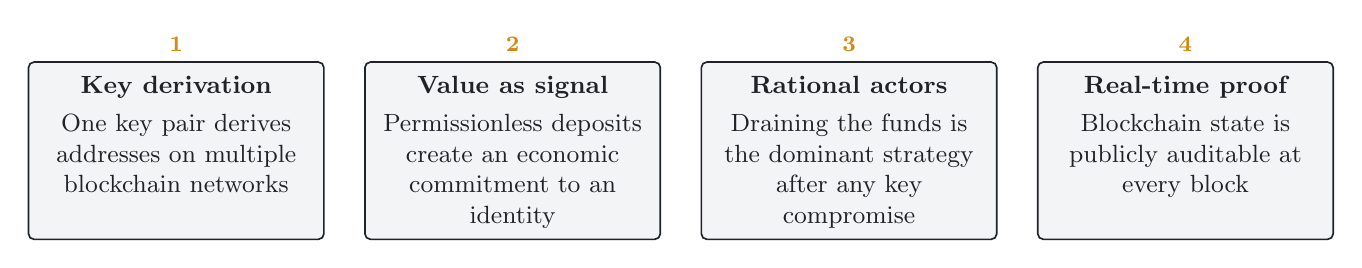
\begin{tikzpicture}[node distance=5mm, pillar/.style={box, anchor=north}]
\node[pillar] (a) at (0,0) {\begin{minipage}[t][19mm][t]{34mm}\centering{\bfseries Key derivation}\\[3pt] One key pair derives addresses on multiple blockchain networks\end{minipage}};
\node[pillar, right=of a.north east, anchor=north west] (b) {\begin{minipage}[t][19mm][t]{34mm}\centering{\bfseries Value as signal}\\[3pt] Permissionless deposits create an economic commitment to an identity\end{minipage}};
\node[pillar, right=of b.north east, anchor=north west] (c) {\begin{minipage}[t][19mm][t]{34mm}\centering{\bfseries Rational actors}\\[3pt] Draining the funds is the dominant strategy after any key compromise\end{minipage}};
\node[pillar, right=of c.north east, anchor=north west] (d) {\begin{minipage}[t][19mm][t]{34mm}\centering{\bfseries Real-time proof}\\[3pt] Blockchain state is publicly auditable at every block\end{minipage}};
\foreach \n/\k in {a/1, b/2, c/3, d/4} \node[font=\footnotesize\bfseries, text=accent, anchor=south] at (\n.north) {\k};
\end{tikzpicture}
\end{document}
